\documentclass[a4paper,12pt,oneside]{article}

\usepackage[utf8]{inputenc}
\usepackage[T1,T2A]{fontenc}
\usepackage[english,russian]{babel}
\usepackage[usenames]{xcolor}
\usepackage{listings}
\usepackage{graphicx}
\usepackage{cmap}
\usepackage{indentfirst}
\usepackage{imakeidx}
\usepackage[unicode]{hyperref}

\hypersetup{
%bookmarks=true,            % show bookmarks bar?
%unicode=false,             % non-Latin characters in Acrobat’s bookmarks
pdfproducer={Producer},    % producer of the document
pdfkeywords={keywords},    % list of keywords
pdfnewwindow=true,         % links in new window
colorlinks=true,           % false: boxed links; true: colored links
linkcolor=black,           % color of internal links
citecolor=black,           % color of links to bibliography
    filecolor=black,           % color of file links
    urlcolor=blue             % color of external links
}

%\begin{lstlisting}[caption={},label={lst:}]
%\end{lstlisting}

\definecolor{olivegreen}{cmyk}{0.64,0,0.95,0.40}
\definecolor{mauve}{rgb}{0.58,0,0.82}

\setlength{\parskip}{6pt}

\lstset{
language=C++,                           % Code langugage
basicstyle=\ttfamily,                   % Code font, Examples: \footnotesize, \ttfamily
keywordstyle=\color{olivegreen},        % Keywords font ('*' = uppercase)
commentstyle=\color{gray},              % Comments font
stringstyle=\color{mauve},
numbers=left,                           % Line nums position
numberstyle=\tiny,
numbersep=10pt,
stepnumber=1,                           % Step between two line-numbers
frame=none,                             % A frame around the code
tabsize=2,                              % Default tab size
captionpos=b,                           % Caption-position = bottom
breaklines=true,                        % Automatic line breaking?
breakatwhitespace=false,                % Automatic breaks only at whitespace?
showspaces=false,                       % Dont make spaces visible
showstringspaces=false,
showtabs=false,                         % Dont make tabls visible
columns=flexible,                       % Column format
title=\lstname,
caption={},
extendedchars=\true,
inputencoding=utf8,
}

\makeindex[intoc]

\title{Память как концепция в гетерогенных системах}
\author{
  Владимиров Константин Игоревич\\
  \texttt{konstantin.vladimirov@gmail.com}
}
\date{\today}

\begin{document}

\begin{titlepage}
\begin{center}

\large ~ \\[4.5cm]

\huge Память как концепция\\[0.6cm]
\large В гетерогенных системах\\[3.7cm]

\begin{minipage}{0.5\textwidth}
\begin{flushleft}
\emph{Автор:} Владимиров К. И.\\
\end{flushleft}
\end{minipage}
\vfill
Email автора: \texttt{konstantin.vladimirov@gmail.com}\\
{\large \today}
{\large \LaTeX}

\end{center}
\thispagestyle{empty}
\end{titlepage}

\tableofcontents

\pagebreak
\section{Введение}\label{sec:Intro}

Гетерогенными системами называются системы, имеющие две выделенных роли: host и device. Host это устройство, которое иницирует вычисления и обрабатывает их результаты, device это устройство, на котором производятся вычисления.
Обычно хост это микропроцессор (CPU) так как исторически именно CPU имеет операционку с которой взаимодействует пользователь, который ставит задачи.
Устройством может быть видеокарточка (GPU), графический ускоритель, специализированная карта для машинного обучения (NPU), другие CPU и даже тот же самый CPU.

\subsection{Программирование GPU и GPGPU}\label{subsec:gpgpu}

Исторически первым опытом человечества в гетерогенном программировании были именно видеокарточки.
Созданные как суперпараллельные устройства с фиксированным графическим конвейером и фиксированным набором управляющих состоянием конвейера переключателей, видеокарточки довольно быстро превратились в нечто большее.
Первые короткие программы, позволяющие нетривиальную обработку вершин (после сборки геометрии) и фрагментов (после растеризатора) использовались в основном для освещения и поэтому назывались вершинными и фрагментными \textbf{шейдерами}.
Довольно скоро оказалось, что такие шейдеры полезны даже если пропустить собственно рендеринг: в параллельном стиле посчитать что-то на GPU систематически оказывалось быстрее и удобнее чем на CPU.

Поскольку шейдеры для графики изначально писались не как программы общего назначения а как специализированные программы для конкретных точек кастомизации, они писались не на языках общего назначения, а на специализированных языках из которых самыми популярными стали GLSL для OpenGL API и HLSL для DirectX API.

И OpenGL и DirectX и многие более поздние API являются именно API -- то есть набором вызовов, доступных программисту для совершения тех или иных действий.
Эти вызовы должны были где-то обрабатываться и формировать запросы к драйверу видеокарточки.
Так возникла концепция \textbf{рантайма}, как промежуточного слоя между пользовательской программой и драйвером.
Один и тот же рантайм может поддерживать несколько разных API и даже делегировать к нижележащим рантаймам.
Например в Intel как OpenCL API так и L0 API поддерживаются одним и тем же NEO runtime (который когда он работает с OpenCL API можно называть OpenCL runtime).

В число поддерживаемых вызовов API неизбежно входит вызов похожий на ``скомпилируй шейдер''. Таким образом неотъемлимой частью рантайма становится \textbf{графический компилятор}.

Первыми опытами в чисто вычислительных задачах исторически стали задачи свёртки (convolution). 
Именно концепция ядра свёртки (convolution kernel) дала название первым небольшим программам для гетерогенных вычислений: их стали называть \textbf{кернелами}.
Ниже везде использование терминов шейдер, кернел и программа будет полностью взаимозаменяемым.
В общем нет ошибки в том, чтобы назвать чисто вычислительную программу шейдером и так далее.

\subsection{О чём пойдёт речь далее}\label{subsec:about}

Структурно всё изложение ниже ведёт к глубокому анализу памяти и работы с ней в SYCL (см. раздел \ref{sec:FiveTasks}).

По пути будут изложены основы памяти для графических API (см. \ref{sec:GPUMEM})., мотивировано использование single-source API для compute (см. \ref{sec:SingleSource}) и дан краткий обзор компиляции и ассемблера для Intel XE (см. \ref{sec:IntelXE}).
Всё это должно помочь понять и воспроизвести соответствующие замеры, в том числе и на доступном читателю железе.
Даже не обязательно на железе Intel XE, так как общие концепции везде одинаковы.

Технический интерес может также представлять изложений концепций атомарности в мире обычного и гетерогенного программирования, к которому изложение придёт в конце, поскольку эти вопросы несколько сложны.

\pagebreak
\section{Структура памяти для графики}\label{sec:GPUMEM}

Основные концепции в программировании графики примерно одинаковые но по разному называются для разных API. Ниже будут использоваться в основном термины из OpenGL и Vulkan -- из-за существенной тяги автора к открытым API. 

Важнейшей концепцией в программировании графики является память обладающая состоянием (stateful memory) и её разновидность: память с общей точкой привязки (bindless memory). 
Несмотря на то, что в языках, ориентированных на вычисления, таких концепций как будто нет, их понимание даёт важные инсайты для того чтобы далее понимать модель памяти, ракладку памяти и даже сгенерированный ассемблер.

\subsection{Память, обладающая состоянием}\label{subsec:stateful}

Ключевые типы памяти это uniform buffer object (UBO) и shared storage buffer object (SSBO). Простое объявление и того и другого проиллюстрировано на (lst. \ref{lst:glslbti}).

\begin{lstlisting}[caption={Простая программа на GLSL с явными binding индексами},label={lst:glslbti}]
struct Particle {
  vec4 pos, vel;
};

layout(std140, binding = 0) buffer Pos {
  Particle particles[];
};

layout (binding = 1) uniform UBO {
  float deltaT; 
  int count;
} ubo;
\end{lstlisting}

Следует обратить внимание на явное указание binding point для буфера. Обычно в GPU есть поддержка в железе для быстрого преобразования binding table index (BTI) и смещения в буфере в физический адрес. В данном случае программист вручную назначил точку с номером ноль для SSBO, а точку с номером один для UBO как показано на (рис. \ref{fig:bti-idea}).

\begin{figure}
\centering
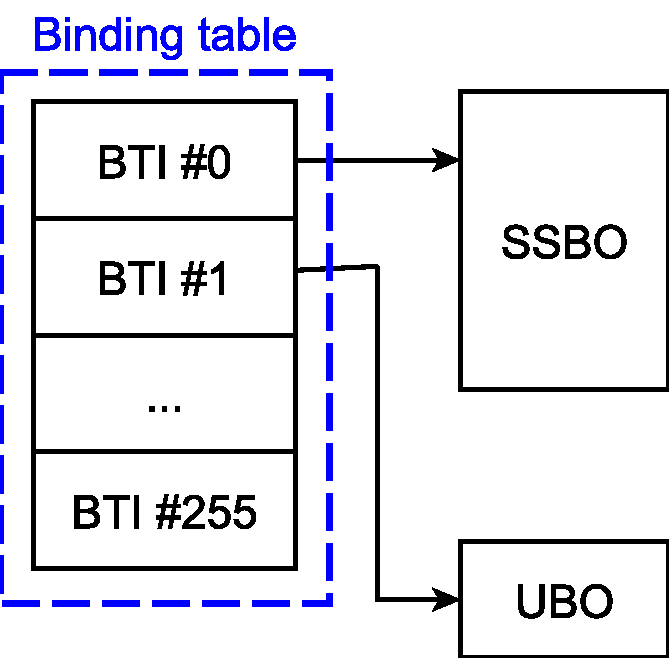
\includegraphics[width=0.5\textwidth]{pictures/bti-idea.pdf}
\caption{Binding table для (lst. \ref{lst:glslbti})}
\label{fig:bti-idea}
\end{figure}

После того как точки привязки назначены, работа с ними ведётся как с обычными массивами, структурами и даже массивами структур (lst. \ref{lst:glslprog}).

\begin{lstlisting}[caption={Работа с UBO и SSBO на GLSL},label={lst:glslprog}]
for (int i = 0; i < ubo.count; i += DataSz)
  if (i + x < ubo.count)
    someData[x] = particles[i + x].pos;
\end{lstlisting}

Но надо очень чётко осознавать: несмотря на то, что адресация \lstinline!particles[i + x]! выглядит похоже на работу с указателями в обычном C или C++, на самом деле это совсем другая концепция. Тут явно указывается буффер с его BTI и смещение в нём. Чтобы понять чем это отличается от настоящих указателей, давайте рассмотрим пример (lst. \ref{lst:glslbad})

\begin{lstlisting}[caption={Отсутствие настоящих указателей в GLSL},label={lst:glslbad}]
int *uboPtr = &ubo.deltaT; // this is not legal GLSL!
int *ssboPtr = &particles[i + x].pos; // and this is either
int *somePtr = CTUnknownCondition() ? ssboPtr : uboPtr;
\end{lstlisting}

Так делать в GLSL нельзя именно потому что наличие указателя как концепции позволяет смешать указатели в выражении, а это потеряет в \lstinline!someptr! информацию о том какой у него номер буфера и какой оффсет в нём.
В итоге компилятор будет просто не в состоянии построить ассемблер для выражения вроде \lstinline!*someptr = 8! так как останется неясно куда записывать восьмёрку.

Такая память, в которой обращение идёт опосредовано -- через BTI и смещение -- называется обладающей состоянием или stateful.
У вас есть незримое состояние: для каждого индекса BTI есть реальный физический адрес куда отображена память и размер буфера по этому адресу, а иногда и нечто другое.
Работа со stateful памятью за счёт аппаратной поддержки может быть очень эффективна, но фактически сырые (то есть stateless) указатели в такой модели оказываются запрещены: они позволяют слишком много.

\textbf{Обсуждение:} как вы думаете что делает stateful указатели более эффективными?
При ответе подумайте над размером stateless указателя в 64-битном адресном пространстве, над отсутствием поддержки 64-битной арифметики во многих видеокартах и над тем насколько эффективней заменить работу с 64-разрядными указателями на работу с 32-разрядными смещениями.

\textbf{Упражнение:} в этом подразделе использован известный пример N-body из
\href{https://github.com/SaschaWillems/Vulkan/blob/master/data/shaders/glsl/computenbody/particle_calculate.comp}{примеров Виллемса для Vulkan API}. Попробуйте скомпилировать его графическим компилятором вашего вендора графики и посмотрите получившийся ассемблер для вашей видеокарточки.

\subsection{Типизированная память}\label{subsec:typedmem}

Многие графические API работают со специальными объектами: изображениями и самплерами. Например (lst. \ref{lst:glslsamplers}) демонстрирует как выход растеризатора смешивается с текстурой и используется для получения итогового цвета фрагмента.

\begin{lstlisting}[caption={Работа с typed памятью},label={lst:glslsamplers}]
layout (binding = 0) uniform sampler2D samplerposition;

layout (location = 0) in vec2 inUV;
layout (location = 0) out vec4 outFragColor;

void main() {
  vec3 fragPos = texture(samplerposition, inUV).rgb;
  vec3 lightPos = vec3(0.0);
  vec3 L = normalize(lightPos - fragPos);
  float NdotL = max(0.5, dot(normal, L));
  outFragColor.rgb = NdotL;
}
\end{lstlisting}

Самое интересное тут это структура памяти текстуры. Очевидно это stateful память, но её state несколько сложнее.
Будучи изображением, текстура хранит свои внутренности в сложном формате, включающем размеры, pitch, цветовую схему.
Самплер как раз призван изолировать нас от этих деталей (а заодно сообщить железу как обрабатывать выходы за пределы текстуры и т.п. чтобы программист не писал этих условий руками).
Такая память, которая скрывает от нас сложные детали каждой своей ячейки, то есть имеет определенный тип ячейки, который снаружи виден как вектор, называется типизированной или \textbf{typed} памятью.

\subsection{Память с единой точкой привязки}\label{subsec:bindless}

Всего точек привязки обычно немного, что-то вроде 255 причём нижние две зарезервированы (например 254 это локальная память и 255 это \textbf{scratch} -- специальная память куда идут выгрузки данных не вместившихся в регистры).
При этом доступных дескрипторов для буферов в Vulkan API могут быть миллионы.

Ещё одна проблема в том, что массив текстур в этой модели нельзя индексировать неизвестным на этапе компиляции значением, так как обращение по оффсету может быть только в пределах одной точки привязки.

Из-за этого в программировании графики возникает концепция памяти с единой точки привязки (bindless memory), доступной, например в GLSL через расширение \lstinline!GL_EXT_nonuniform_qualifier!.

\begin{lstlisting}[caption={Работа с bindless памятью на GLSL},label={lst:bindless}]
#extension GL_EXT_nonuniform_qualifier : enable
layout (set = 1, binding = 10) uniform sampler2D textures[];
// ....
vec4 color = texture(textures[albedo_id], final_uv.xy);
\end{lstlisting}

Здесь \lstinline!albedo_id! может быть неизвестен на этапе компиляции, но это не так важно: весь массив, как показано на (рис. \ref{fig:bti-idea}) привязан к одной точке привязки и далее в пределах массива возможна индексация.
Эта концепция несколько приближает смещение в таком массиве к настоящему указателю, а сам массив -- к специальному адресному пространству к которому этот указатель принадлежит.

\begin{figure}
\centering
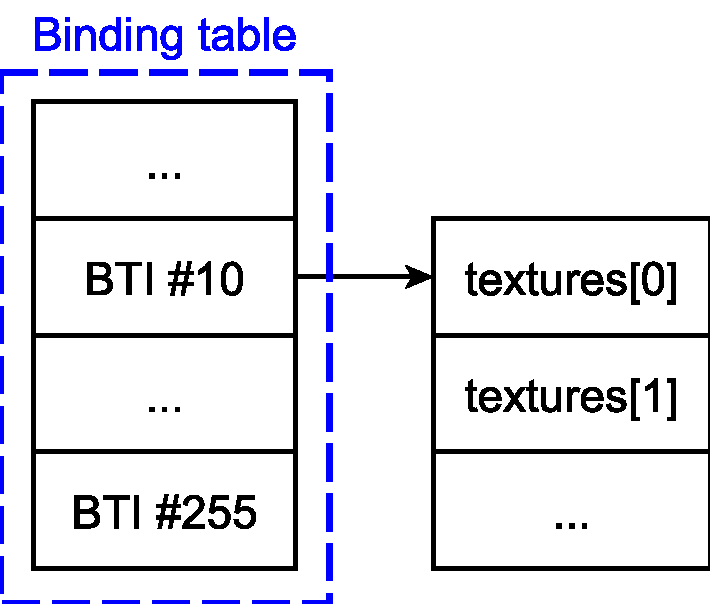
\includegraphics[width=0.5\textwidth]{pictures/bindless-idea.pdf}
\caption{Концепция bindless памяти для (lst. \ref{lst:bindless})}
\label{fig:bindless-idea}
\end{figure}

Главная претензия к отсутствию настоящих указателей: невозможность просто на оффсетах и буферах делать удобные дианмические структуры данных.
Конечно можно представить дерево или даже граф закодированные как линейный массив, но вряд ли операции над таким представлением будут сохранять асимптотическую эффективность.

\subsection{Конвергенция 3D: device pointers}\label{subsec:devpointers}

Графика постоянно приближается по мощности работы с памятью к вычислительным языкам, свидетельством чему является появившееся недавно расширение \lstinline!GLSL_EXT_buffer_reference!, работа с которым показана на (lst. \ref{lst:devptrs}).

\begin{lstlisting}[caption={Работа с device pointers на GLSL},label={lst:devptrs}]
// forward declaration
layout(buffer_reference) buffer blockType;

layout(buffer_reference, std430, buffer_reference_align = 16) 
buffer blockType {
  int x;
  blockType next;
};

layout(std430) buffer rootBlock {
  blockType root;
} r;

void main() {
  blockType b = r.root;
  // "pointer chasing" through a linked list
  b = b.next.next.next.next.next;
}
\end{lstlisting}

Тем не менее, даже такое совершенное приближение к концепции указателя не даёт ответа на фундаментальный вопрос: как быть с отображением указателей? 

Допустим мы находимся в мире гетерогенного программирования и у нас есть хост, который подготовил дерево, связный список или граф и куча устройств, которые готовы с этой структурой данных работать.
Можем ли мы прозрачно, указатель в указатель, отобразить эту структуру данных на устройство, не переделывая указатели в узлах?

То есть, шире говоря, возможно ли работать с памятью хоста и памятью одного или нескольких устройств как с унифицированной виртуальной памятью?

\pagebreak
\section{Вычислительные API}\label{sec:SingleSource}

Первые вычислительные API были разновидностью API для графики и до сих пор и OpenGL compute и Vulkan compute отлично существуют.
Их применимость ограничена их моделью памяти.
Кроме того они по уважительным причинам имеют чёткую границу между кодом для устройства и кодом для хоста.
Вы пишете хостовую программу и для неё код вашего шейдера это не код это кусок текста.
Это выглядит неплохо для графики, где шейдер не особо общается с хостовым кодом, а зависит в основном от выхода таких слабо контролируемых программистом устройств как сборщик геометрии или растеризатор.
Но что лучше подходит для вычислений?

\subsection{OpenCL}\label{subsec:opencl}

Появившийся в 2009-м году стандарт OpenCL (сравните с 1992-м годом OpenGL) ознаменовал начало эры программирования General Purpose GPU (или GPGPU), из которого потом вырос целый мир гетерогенного программирования.
Строго говоря, CUDA появилась в 2007-м, что несколько раньше, но, вспомним, что автор питает сильное пристрастие к открытым API, а CUDA сильно залочена на NVidia и имеет ряд других особенностей о которых ниже.
Будучи первым открытым compute API, OpenCL, разумеется, был сделан со всеми оглядками на существующие графические API, то есть separate-source. В общем и немудрено: семнадцать лет развития графики давали неплохую инерцию мышления.

Единицей работы с памятью в OpenCL является \textbf{буфер}.
Хостовая программа запрашивает у рантайма OpenCL создание буфера либо через явный вызов API, такой как clCreateBuffer, либо в более совершенном C++ API просто в конструкторе reference-counted RAII объекта.
Точно так же для пересылки есть явные API вроде clEnqueueReadBuffer, но, разумеется, лучше когда их просто вызывает под капотом алгоритм \lstinline!cl::copy!, как это показано на (lst. \ref{lst:oclbuf}).

\begin{lstlisting}[caption={Пересылка буфера, OpenCL},label={lst:oclbuf}]
cl::vector<int> A(BUFSZ), B(BUFSZ);
cl::Context Context{CL_DEVICE_TYPE_GPU, properties};
cl::CommandQueue Queue{Context};

// Buffer D on device
cl::Buffer D{Context, CL_MEM_READ_WRITE, BUFSZ * sizeof(int)};

// Send A to D (from host to device)
cl::copy(Queue, A.begin(), A.end(), D);

// Send D to B (from device back to host)
cl::copy(Queue, D, B.begin(), B.end());
\end{lstlisting}

С одной стороны буфер как идея напоминает нам BTI из графики. С другой стороны, простая программа на OpenCL C, которая работает с буферами, оперирует в качестве своих аргументов аннотированными указателями, как это показано на (lst. \ref{lst:oclvadd}).

\begin{lstlisting}[caption={Векторное сложение, OpenCL},label={lst:oclvadd}]
__kernel void
vector_add(__global int *A, __global int *B, __global int *C) {
  int i = get_global_id(0);
  C[i] = A[i] + B[i];
}
\end{lstlisting}

С точки зрения кода на C++ это просто текст и создание из него функтора происходит в рантайме.
Опять-таки можно использовать низкоуровневые вызовы clBuildProgram и т.п., можно проделать это более человечно в конструкторе RAII-объекта, как показано на (lst. \ref{lst:oclkern}).

\begin{lstlisting}[caption={Создание кернела, OpenCL},label={lst:oclkern}]
cl::Context Context{CL_DEVICE_TYPE_GPU, prop};
cl::CommandQueue Queue{Context};

// true == build immediately
cl::Program program{Context, vakernel, true};

cl::NDRange GlobalRange{Sz};
cl::EnqueueArgs Args{Queue, GlobalRange};
using KernTy = cl::KernelFunctor<cl::Buffer, cl::Buffer, cl::Buffer>;
KernTy add_vecs{program, "vector_add"};

// enque, execute, wait
cl::Event evt = add_vecs(Args, A, B, C);
\end{lstlisting}

На (рис. \ref{fig:oclkern}) показана схема того, что происходит с текстом программы когда он попадает в жернова рантайма и графического компилятора.
Программа обрабатывается фронтендом (часто clang-based) до стабильного промежуточного представления (стандарт де-факто это SPIRV, но могут быть варианты).
Далее подключается оптимизатор, который делает из бинарника в стабильном промежуточном представлении бинарник для конкретного устройства на котором исполняется программа.

\begin{figure}
\centering
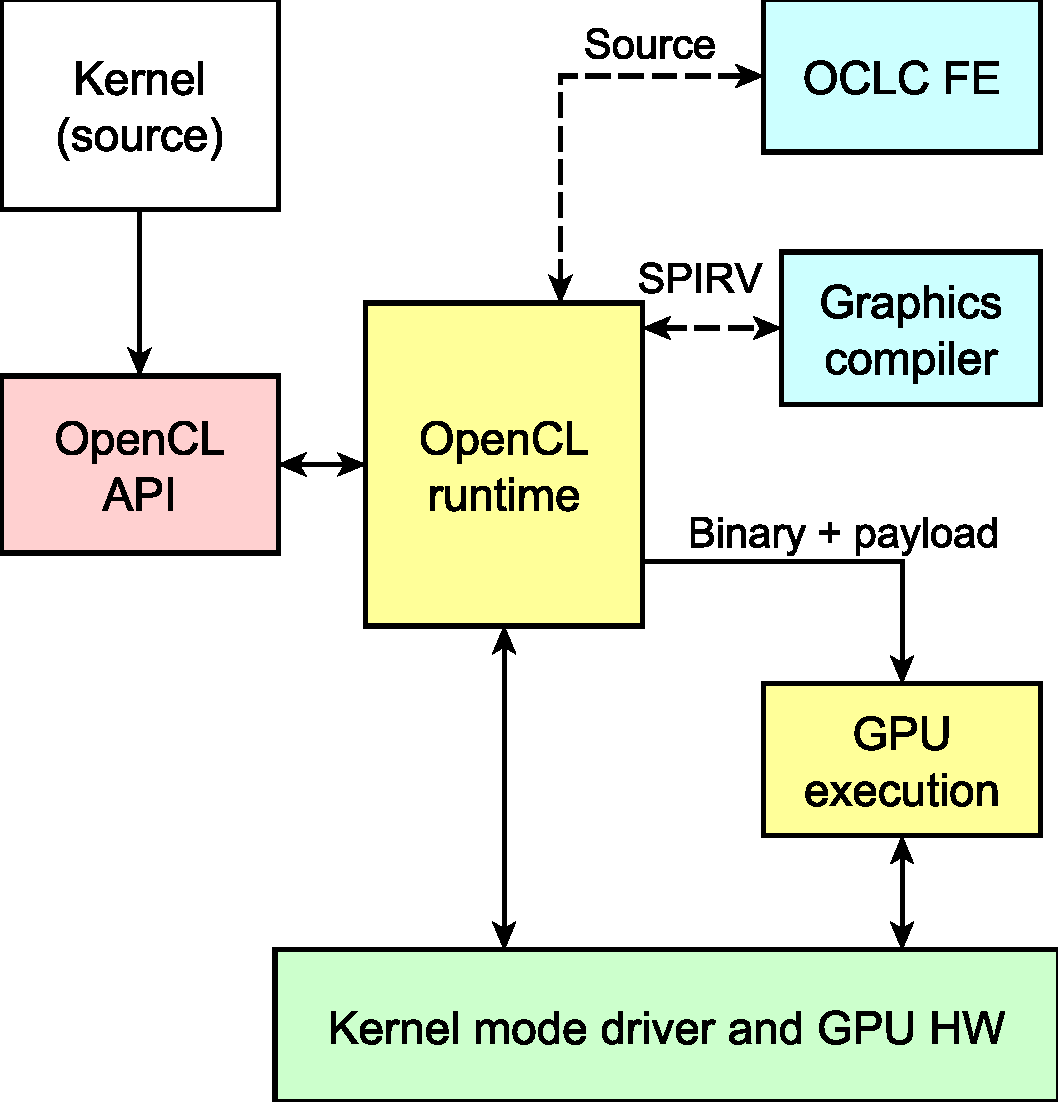
\includegraphics[width=0.5\textwidth]{pictures/ocl-compilation-scheme.pdf}
\caption{Схема компиляции для (lst. \ref{lst:oclkern})}
\label{fig:oclkern}
\end{figure}

Разумеется не обязательно подавать текстовый файл и проходить все эти этапы.
OpenCL API позволяет вызывать и CreateProgramFromText и CreateProgramFromIL и даже CreateProgramFromBinary.
В последнем случае речь идёт об Ahead Of Time (AOT) компиляции, в первых двух случаях о разных версиях Just in Time (JIT) компиляции.
В случае AOT компиляции вы должны быть уверены что платформа и версия бинарного файла совпадут с вашим вычислительным устройством.

\subsection{CUDA, OpenMP, SYCL}\label{subsec:typesafety}

У API с раздельным исходным кодом есть фундаментальная проблема для вычислительных задач.
Поскольку они напрямую взаимодействуют с хостом (по сути они притворяются функциями, вызываемыми с хоста) у них есть границы интерфейсов.

Но хост не может проконтролировать безопасность типов по этим границам. Пример (lst. \ref{lst:oclvadd}) с точки зрения хостового кода выглядит как показано на (lst. \ref{lst:oclvaddhost}) то есть довольно-таки безнадёжно.

\begin{lstlisting}[caption={Векторное сложение, OpenCL c точки зрения хоста},label={lst:oclvaddhost}]
const char *vakernel = "__kernel void vector_add("
" __global int *A, __global int *B, __global int *C) {"
" int i = get_global_id(0);"
" C[i] = A[i] + B[i];"
"}";
\end{lstlisting}

\textbf{Обсуждение:} чему равен sizeof(int) на вашей графической карте и сколько вы будете отлаживать ошибку, если он не совпадёт с хостовым?

Разумеется есть много ухищрений на которые тут можно пойти, например использовать всюду \lstinline!cl_int!, для которого совпадение размеров гарантированно.
Но давайте будем честны: если у вас есть массив структур из двух int, вы вряд ли будете перекладывать его в массив структур из двух \lstinline!cl_int!.
Скорее уж вы будете надеяться что всё будет работать, у вас же на машине работает.
А даже если и переложите, то всё равно вам останется только молиться, чтобы совпало выравнивание.

Человечество осознало эту проблему довольно рано и первым single-source API стала CUDA в 2007-м году. После CUDA появился SYCL в 2014-м, и возможность оффлоада на гетерогенные устройства была добавлена в стандарт OpenMP.

Основной проблемой для single-source API является то, что обычный C++ не подходит для выражения ряда важных концепций. В нём нет разных типов памяти, нет интерфейсов для оффлоада и многого другого. Итак, что же можно сделать, чтобы решить эту проблему?

\textbf{Первый вариант:} расширить C++ новыми ключевыми словами и синтаксическими элементами. 

По этому пути изначально пошла CUDA, см. (lst. \ref{lst:cudavadd}) и он кажется наиболее простым.
Но на самом деле он порождает массу сложностей: если мы пишем не вполне на C++, насколько, собственно идиомы и соглашения C++ приложимы к тому, на чём мы пишем?
Как оно будет эволюционировать с новыми стандартами?
Можем ли мы судить о поведении всей программы, например при ODR violation для кернелов?

\begin{lstlisting}[caption={Векторное сложение, CUDA},label={lst:cudavadd}]
__global__ void vecAdd(int *A, int *B, int *C, int N);
....
cudaMalloc((void **)&a_d, n * sizeof(int));
cudaMalloc((void **)&b_d, n * sizeof(int));
cudaMalloc((void **)&c_d, n * sizeof(int));
vecAdd<<<block_no, block_size>>>(a_d, b_d, c_d, n);
\end{lstlisting}

Конечно, если рано или поздно это удастся протащить в стандарт, эти вопросы будут сняты, но пока что кажется до этого далеко.
Да и корпорация NVidia, судя по их лицензии, явно не хочет видеть альтернативных реализаций CUDA.

\textbf{Второй вариант:} расширить C++ новыми прагмами.

Этот путь выбрали в OpenMP, для примера см. (lst. \ref{lst:ompred}).
Причём этот выбор был сделан задолго до привнесения в OpenMP самой возможности делать оффлоады.
Оно изначально было так спроектировано.

\begin{lstlisting}[caption={Редукция, OpenMP},label={lst:ompred}]
#pragma omp target parallel private(ompSum) shared(totalSum)
{
  ompSum = 0;

  #pragma omp for
  for (int i = 0; i < N; i++)
    ompSum += array[i];

  #pragma omp critical
  totalSum += ompSum;
}
\end{lstlisting}

Здесь те же возражения в несколько ослабленном виде.
Являясь нестандартными конструкциями, прагмы притворяются что их нет.
Но объекты, на которые они влияют, нетривиально взаимодействуют с объектами, подчиняющимися стандарту.
Возьмём прагму \lstinline!shared(totalSum)! -- она как минимум изменяет область видимости, время жизни и правила synchronized-with для аннотируемой переменной.
Язык C++ достаточно сложен сам по себе, чтобы не перегружать его дополнительной семантикой такого рода.
Кроме того субъективно это критично ухудшает читаемость кода (впрочем это не аргумент).

\textbf{Третий вариант:} не трогать C++, обойтись библиотечной поддержкой.

Это путь по которому пошёл, например, SYCL см. (lst. \ref{lst:syclfn}).
Ключевая развязка хостового кода с кодом устройства осуществляется через взятую из OpenCL концепцию очереди.

\begin{lstlisting}[caption={Выполнение DeviceFn, SYCL},label={lst:syclfn}]
auto Event = Queue.submit(
  [&](sycl::handler &Cgh) {
    // .....
    Cgh.parallel_for<name>(Range, DeviceFn);
  });
\end{lstlisting}

Но в очередь ставится не конкретная функция, а command group: кернел плюс его зависимости. На (рис. \ref{fig:syclfn}) показано как это может происходить.

\begin{figure}
\centering
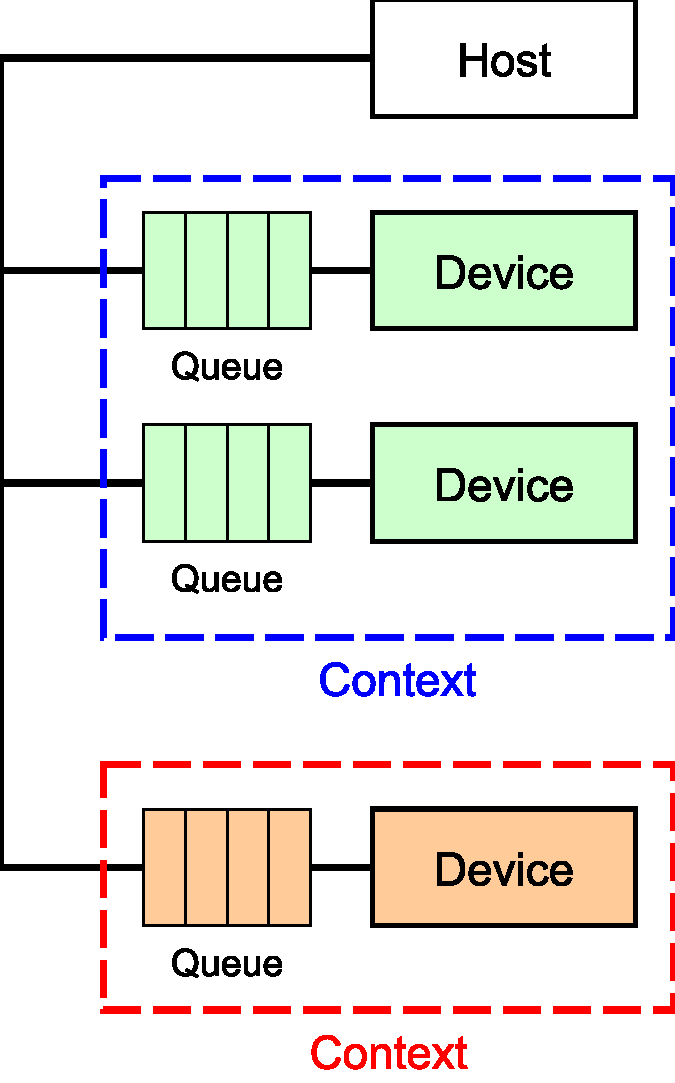
\includegraphics[width=0.5\textwidth]{pictures/hetero-prog-queue.pdf}
\caption{Схема постановки в очередь для (lst. \ref{lst:syclfn})}
\label{fig:syclfn}
\end{figure}

Устройства, имеющие один и тот же компилятор, один и тот же бинарный формат (например два GPU одного вендора) могут быть объединены в контекст. Простейший контекст это единственное устройство. Далее кернел, скомпилированный в контексте может быть поставлен в очередь на одно из его устройств.
При этом поддерживается сквозная типизация, что уберегает от ошибок из-за несогласованности размеров и прочего.

Далее для всех примеров будет использоваться SYCL.
Главная задача дальнейшего изложения это показать как память в гетерогенных системах соотносится с обычной памятью в обычных программах на C++.
Проще всего это достигается при рассмотрении конкретных примеров.
Но чтобы рассматривать конкретные примеры надо договориться о конкретной архитектуре.

\pagebreak
\section{Компиляция OneAPI и ассемблер Intel XE}\label{sec:IntelXE}

Сейчас самый удобный способ писать на SYCL это использование Intel OneAPI.
Несмотря на то что производительность (зачастую встроенных) видеокарт Intel пока что отстаёт от лучших образцов дискретной графики NVidia, они широко распространены и многие задачи на них удивительно эффективны (особенно после 12-го поколения).
Бэкенды SYCL для других видеокарт (в том числе NVidia и AMD) существуют, но проигрывают специализированным средствам.
А для Intel, компилятор SYCL из поставки OneAPI это и есть специализированное средство, максимально оптимизируемое под доступное железо.

Для того, чтобы исследовать ассемблер и поэтапную компиляцию, лучше использовать какой-нибудь очень простой пример.
Классический пример не очень полезной, но максимально простой задачи это сложение векторов (см. \ref{lst:syclvadd}).

\begin{lstlisting}[caption={Сложение векторов на SYCL},label={lst:syclvadd}]
// allocate shared memory, common for device and host
auto *A = cl::sycl::malloc_shared<T>(Sz, Queue);
auto *B = cl::sycl::malloc_shared<T>(Sz, Queue);
auto *C = cl::sycl::malloc_shared<T>(Sz, Queue);

// copy to shared memory
std::copy(AVec, AVec + Sz, A);
std::copy(BVec, BVec + Sz, B);

// offload and wait (here GPU computation may happen)
Queue.parallel_for(cl::sycl::range<1>{Sz},
                   [=](auto n) { C[n] = A[n] + B[n]; });
Queue.wait();

// copy back from shared memory
std::copy(C, C + Sz, CVec);

// free shared memory 
cl::sycl::free(A, Queue);
cl::sycl::free(B, Queue);
cl::sycl::free(C, Queue);
\end{lstlisting}

Схема компиляции включает:

\begin{itemize}
\item \textbf{SYCL compiler}, который разделяет исходники на код для хоста и устройства и компилирует код устройства до стабильного промежуточного представления (SPIRV).
\item \textbf{Graphics compiler}, который конвертирует SPIRV в LLVM IR и оптимизирует IR до генерации бинарника устройства. 
\item \textbf{Compute Runtime}, который взаимодействует с OpenCL API, устанавливает значения аргументов, включая неявные и более того.
\end{itemize}

\subsection{От исходников до SPIRV}\label{subsec:syclcompiler}

Результатом работы компилятора SYCL является хостовый бинарник с секциями SPIRV. Для этого, как показано на (рис. \ref{fig:syclscheme}) компилятор должен разделить единый исходник на часть с кодом для хоста и часть с кодом для устройства.

\begin{figure}
\centering
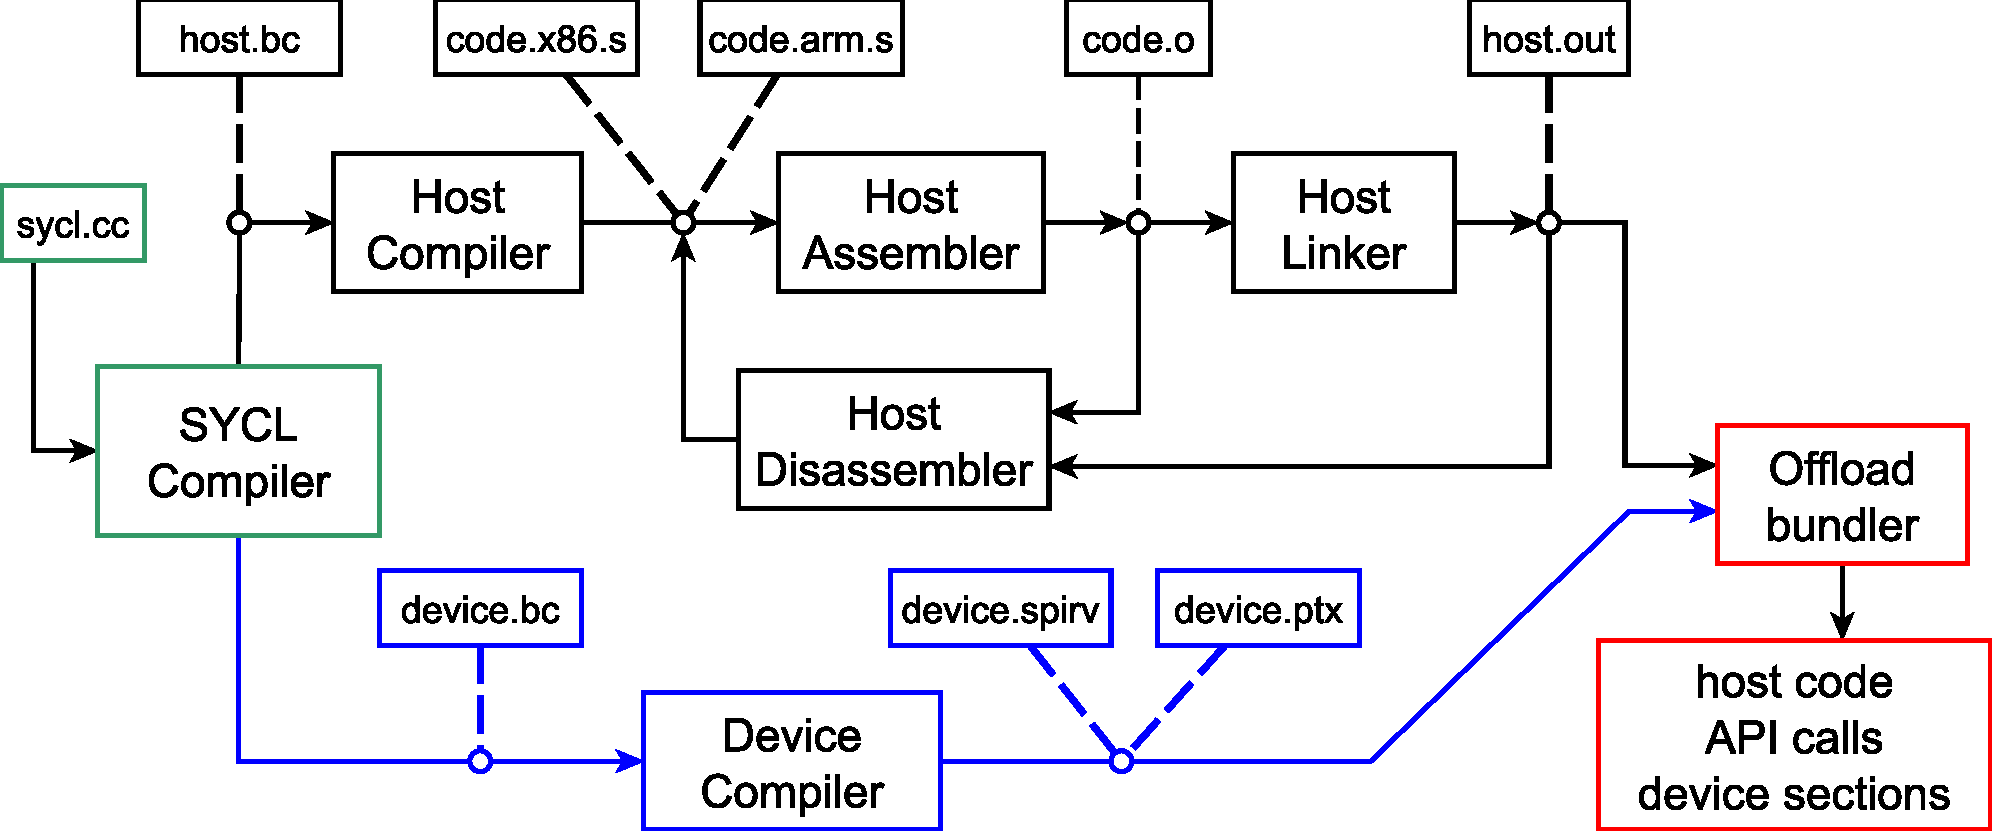
\includegraphics[width=1.1\textwidth]{pictures/sycl-scheme.pdf}
\caption{Схема компиляции до бинарника со SPIRV секциями}
\label{fig:syclscheme}
\end{figure}

\subsection{От SPIRV до VISA}\label{subsec:igc}

\pagebreak
\section{Пять главных задач на SYCL}\label{sec:FiveTasks}

Каждый из примеров ниже относится к числу самых распространённых программ, отдаваемых на видеокарточки.
И каждый из них может научить чему-то важному.
Разумеется начать (и ввести все концепции, которые надо ввести) следует с перемножения матриц.
Для GPGPU это задача задач и выполняя её хорошо, можно сделать очень и очень много практически важных вещей.

\subsection{Перемножение матриц}\label{subsec:gemm}
% \subsection{Битоническая сортировка}\label{subsec:bitonic}
% \subsection{Свёртки}\label{subsec:convolution}
% \subsection{Гистограмма}\label{subsec:hist}
% \subsection{Редукции}\label{subsec:reduction}

% \section{Атомарность в SYCL и в C++}\label{sec:Atomicity}

\end{document}
